 \documentclass[11pt,a4paper,onecolumn]{article}
% \documentclass[options]{class}
% Example: \documentclass[11pt,twoside,a4paper]{article} 10 pt is by default.

\setlength{\columnsep}{1cm}
 

\usepackage[T1]{fontenc}       % Use modern font encodings
% \usepackage[version=3]{mhchem} % Formula subscripts using \ce{}
\usepackage{graphicx}
\usepackage[a4paper,top=2cm, bottom=2.5cm, left=2.5cm, right=2.5cm]{geometry}
% \usepackage{authblk} % For affiliation. This package is not preinstalled.
\graphicspath{{./sup_info/}}
\newcommand*\commentauthor[1]{\textbf{{\textit{#1}}}}
\newcommand*\me[1]{\ensuremath{\bar{#1}\,}}
\newcommand*\chem[1]{\ensuremath{\mathrm{#1}}}

\newcommand*{\affaddr}[1]{#1} % No op here. Customize it for different styles.
\newcommand*{\affmark}[1][*]{\textsuperscript{#1}}
\newcommand*{\email}[1]{\texttt{#1}} % These three commands are for author affilations.

\linespread{1.3} % Line spacing. 1.3 means one-and-a-half spacing.

\begin{document}

%\author{
%Weichun Zhang, Mart\'in Caldarola, Biswajit Pradhan, Michel Orrit\\\affaddr{Huygens-Kamerlingh Onnes Laboratory, Leiden University, 2300 RA Leiden, Netherlands}\\\email{orrit@physics.leidenuniv.nl}
%}

\date{\vspace{1ex}} % Exclude date in the title.
%\affiliation
 %\affil{Huygens-Kamerlingh Onnes Laboratory, Leiden University, 2300 RA Leiden, Netherlands} % This is only useful for authblk package.
 %\email{orrit@leidenuniv.nl}
\title{\textbf{Electrochemsitry of single Azurin shows time variant turnovers}\\ \vspace{3ex} Supplementary Information \vspace{3ex}}
\maketitle
\tableofcontents
\pagebreak

\section{Time traces}

\begin{figure}
  \centering
  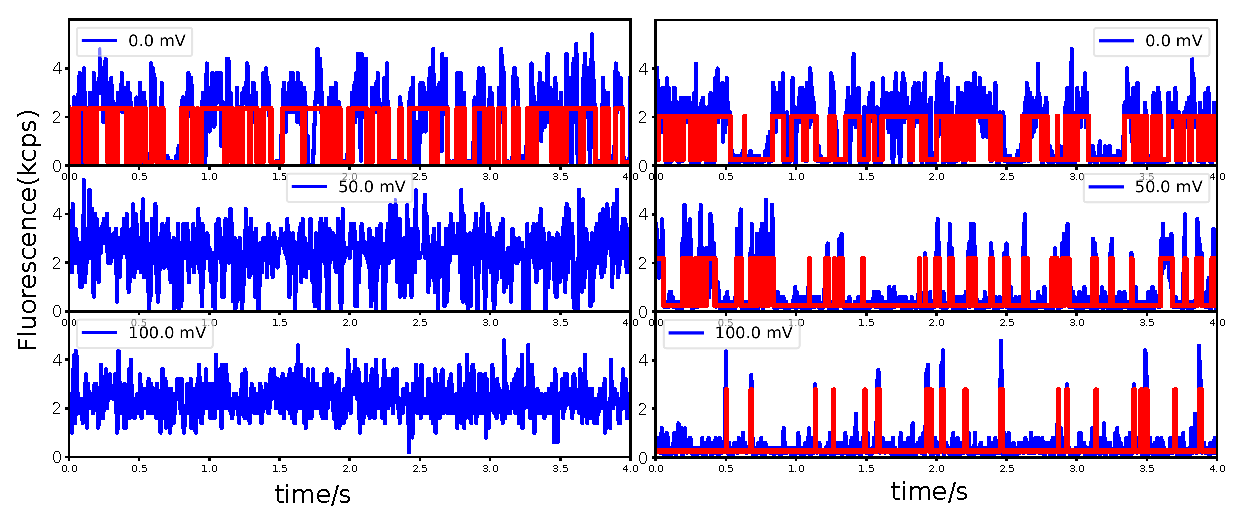
\includegraphics[width=\textwidth,keepaspectratio]{Figure_SI/SI_timetrace_Zn_Cu.eps}
	\makeatletter
	\renewcommand{\fnum@figure}{\figurename~S\thefigure}
	\makeatother
  \caption{Time traces of Zn Azurin (left) and of Cu Azurin(right)}
  \label{fg:NR_coating}
\end{figure}

%\bibliography{}


\end{document}
